\documentclass[12pt,a4paper]{scrartcl}
\usepackage[utf8]{inputenc}
\usepackage[english,russian]{babel}
\usepackage{amssymb,amsfonts}
\usepackage{amsmath,cite,enumerate}
\usepackage{float,indentfirst}
\usepackage{graphicx}
\usepackage{geometry} % Меняем поля страницы
\geometry{left=2cm}% левое поле
\geometry{right=1.5cm}% правое поле
\geometry{top=1cm}% верхнее поле
\geometry{bottom=2cm}% нижнее поле
\graphicspath{{images/}}

\begin{document}


\begin{titlepage}
  \begin{center}
    Санкт-Петербургский Политехнический Университет     Петра Великого \\
    
    Институт компьютерных наук и технологий \\
    
    Кафедра компьютерных систем и программных технологий
  \end{center}
  
  \vfill
  
  \begin{center}
  Лабораторная работа №1\\
  по теме\\
  "Сигналы телекоммуникационных
систем"\\
\end{center}

\vfill

\newlength{\ML}
\settowidth{\ML}{«\underline{\hspace{0.7cm}}» \underline{\hspace{2cm}}}
\hfill\begin{minipage}{0.4\textwidth}
  Выполнил студент группы 33501/3\\
  \underline{\hspace{\ML}} Кисличенко Б.\,Д\\
\end{minipage}%

\bigskip

\settowidth{\ML}{«\underline{\hspace{0.7cm}}» \underline{\hspace{2cm}}}
\hfill\begin{minipage}{0.4\textwidth}
  Руководитель\\
  \underline{\hspace{\ML}} Богач Н.\,В\\
\end{minipage}%

\vfill
 
\begin{center}
  Санкт-Петербург\\
2018 
\end{center}

\end{titlepage}

\section{Цель}
\label{sec:goal}

Познакомиться со средствами генерации сигналов и визуализации их спектров.\\

\section{Постановка задачи}
\label{sec:task}

В командном окне MATLAB и в среде Simulink промоделировать синусоидальный и прямоугольный сигналы с различными параметрами. Получить их спектры. Вывести на график.\\

\section{Теоретический раздел}
\label{sec:teoriya}
Как известно,очень важную роль в технике обработки сигналов играют \textbf{гармонические} сигналы, которые записываются следующим способом:
$$s(t)=A\cos (\omega t+\varphi _0),$$ где  A - амлитуда колебаний, $\omega$ - циклическая (круговая) частота, $\varphi _0$ - начальная фаза, $\varphi = \omega t+\varphi _0$ - фаза колебаний.

\textbf{Амплитуда колебаний} — это абсолютная величина максимального отклонения колеблющейся точки от положения равновесия.

\textbf{Фаза колебаний} – это аргумент периодической функции, описывающей колебательный процесс. Фаза колебания показывает, какая часть периода прошла с момента начала наблюдения колебаний. При заданной амплитуде фаза колебаний полностью определяет смещение колеблющегося тела в любой момент времени.

\textbf{Начальная фаза колебаний} – это фаза колебаний в начальный момент времени t=0. 

\textbf{Период колебаний (сек.)} – это время, за которое тело совершает одно полное колебание. 

\textbf{Частота колебаний (Гц)} – это число колебаний, совершаемых телом в единицу времени:
$$ \nu = \frac{n}{T} = \frac{1}{T}$$

\textbf{Циклическая частота (рад/с)} – это число колебаний, совершаемых телом за $2\pi$ секунд: 
$$\omega = \frac{2\pi}{T} = 2\pi \nu$$

\textbf{Меандр} - это прямоугольный сигнал, у которого длительность импульса и паузы равны. Обычный прямоугольный сигнал отличается от меандра тем, что имеет разную длительность импульса и паузы. 

\begin{figure}[h!]
\center{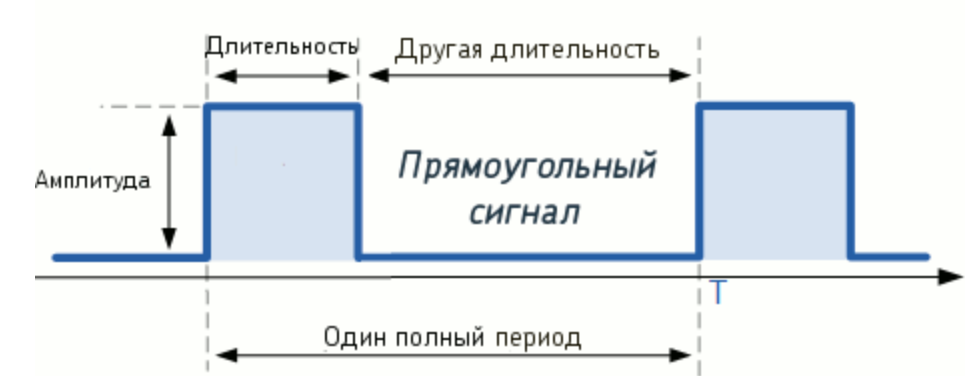
\includegraphics[width=0.6\linewidth]{teoria_pryam_signal}}
\caption{Параметры прямоугольного сигнала}
\end{figure}

Прямоугольные сигналы можно охарактеризовать \textbf{скважностью} (S) и \textbf{коэффициентом заполнения} (D):

$$S=\frac{T}{\tau}=\frac{1}{D}$$

Совокупность амплитуд гармоник ряда Фурье часто называют \textbf{амплитудным спектром}, а совокупность их фаз - \textbf{фазовым спектром}.

Разложению в ряд Фурье могут подвергаться периодические сигналы. При этом представляются в виде суммы гармонических функций либо комплексных экспонент с частотами, образующими арифметическую прогрессию. Для того, чтобы такое разложение существовало, фрагмент сигнала длительностью в один период должен удовлетворять условиям Дирихле:\\
1) Не должно быть разрывов второго рода ( с уходящими в бесконечность ветвями функциями);\\
2) Число разрывов первого рода (скачков) должно быть конечным;\\
3)Число экстремумов должно быть конечным.

Комплексная форма записи ряда Фурье:
$$s(t)=\sum_{k=-\infty}^\infty C_k e^{-jk\omega t}$$

Комплексные коэффициенты ряда связаны с амплитудами $A_k$ и фазами $\varphi _k$, фигурирующими в вещественной форме записи ряда Фурье, следующими соотношениями:

$$C_k = \frac{1}{2}A_k e^{j\varphi k},$$

$$A_k = 2|C|_k|$$

Формула прямого преобразования Фурье:

$$S(\omega) = \int_{-\infty}^\infty s(t) e^{-j\omega t} dt$$

Чтобы преобразование Фурье было применимо, сигнал должен удовлетворять следующим требованиям:

1) должны выполняться условия Дирихле;\\
2) сигнал должен быть абсолютно интегрируемым. Это означает, что интеграл от его модуля должен быть конечной величиной:

$$\int_{-\infty}^\infty|s(t)|dt<\infty$$

Однако с привлечением математического аппарата обобщенных функций возможно выполнение Фурье-анализа и для некторых сигналов, не удовлетворяющим этим требованиям.
\\

\newpage

\section{Ход работы}
\label{sec:work}

\subsection{Работаем в Matlab}
\label{sec:workMatlab}
%Рисунок 2
\begin{figure}[h!]
\center{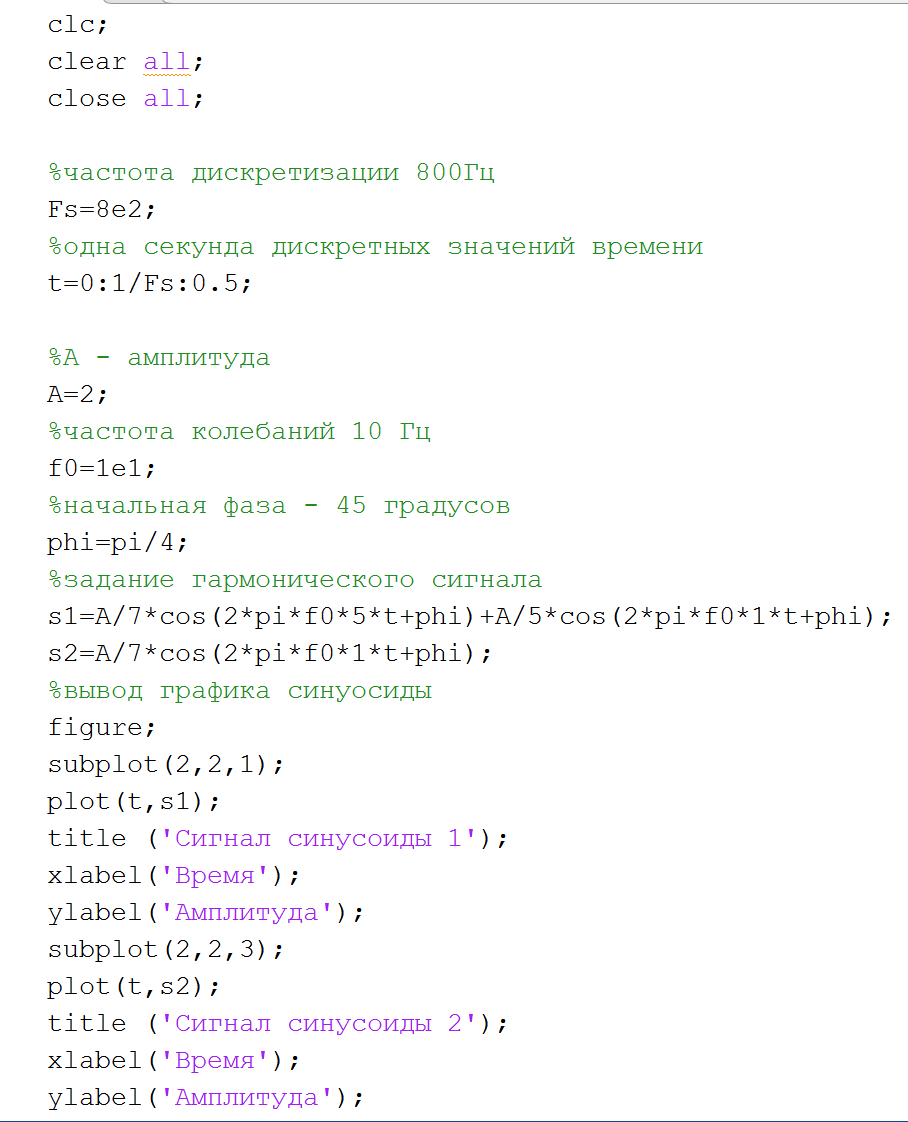
\includegraphics[width=0.9\linewidth]{sin_signal1}}
\caption{Генерируем два синусоидальных сигнала}
\end{figure}

%Рисунок 3
\begin{figure}[h!]
\center{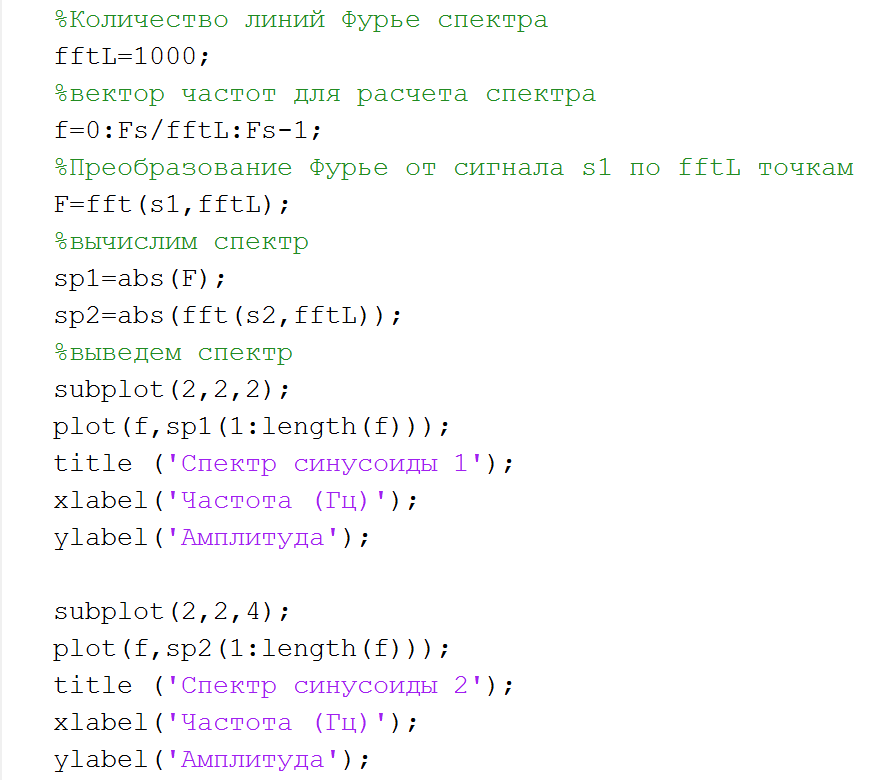
\includegraphics[width=0.9\linewidth]{sin_signal2}}
\caption{Получаем спектры двух синусоидальных сигналов}
\end{figure}

%Рисунок 4
\begin{figure}[h!]
\center{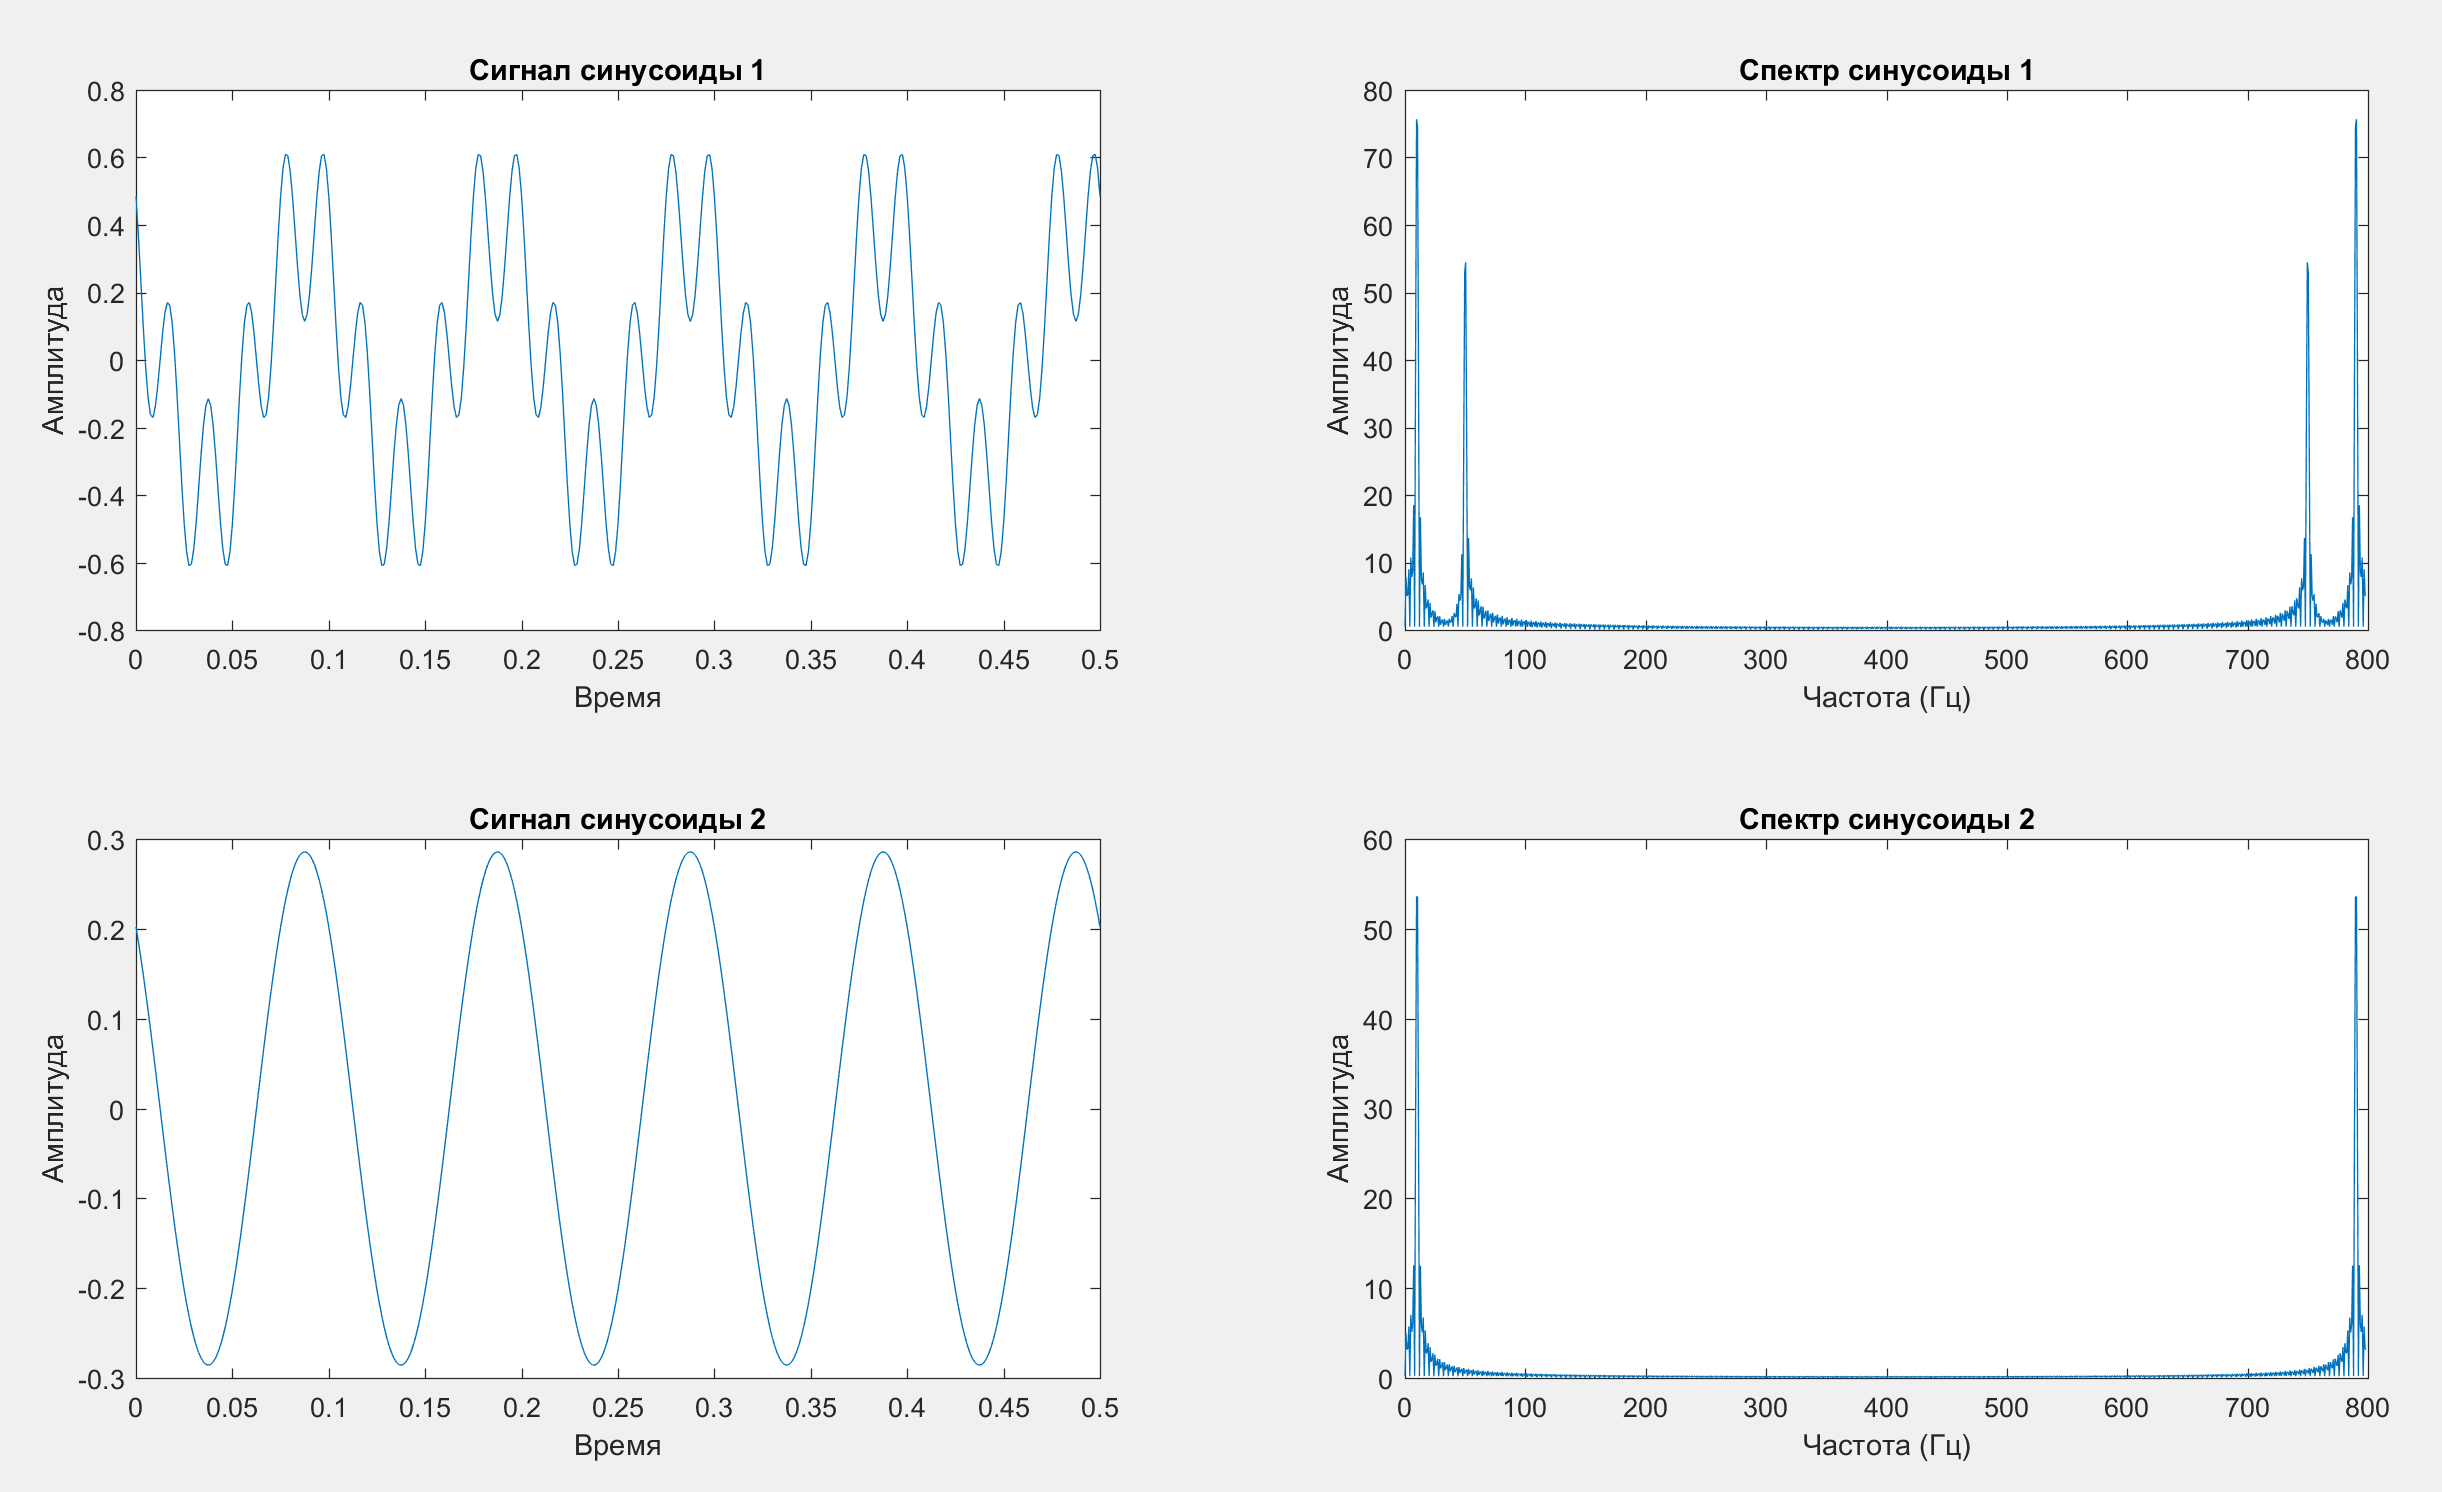
\includegraphics[width=0.9\linewidth]{sin_out}}
\caption{Вывод синусоид и их спектров}
\end{figure}
\newpage

%Рисунок 5
\begin{figure}[h!]
\center{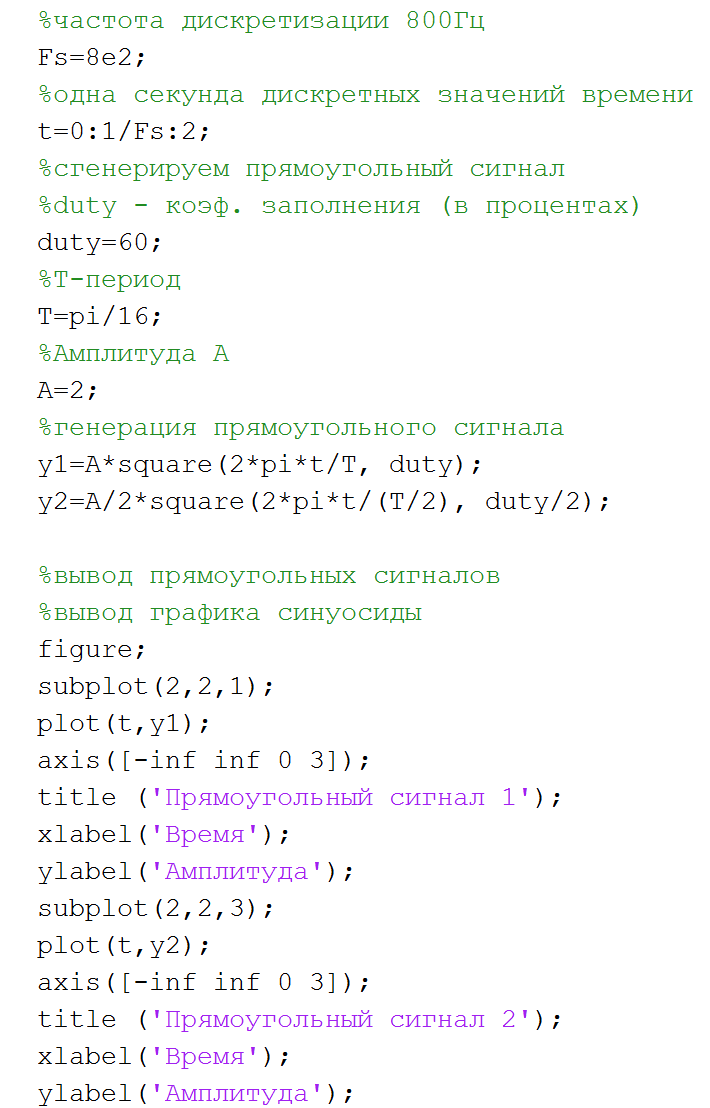
\includegraphics[width=0.9\linewidth]{square_signal1}}
\caption{Генерируем два прямоугольных сигнала}
\end{figure}
\newpage


%Рисунок 6
\begin{figure}[h!]
\center{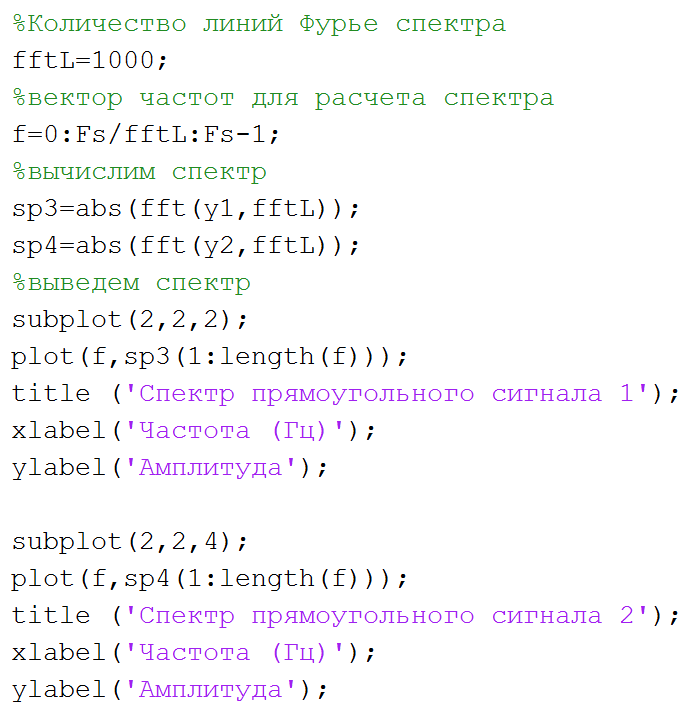
\includegraphics[width=0.9\linewidth]{square_signal2}}
\caption{Получаем спектры двух прямоугольных сигналов}
\end{figure}

%Рисунок 6
\begin{figure}[h!]
\center{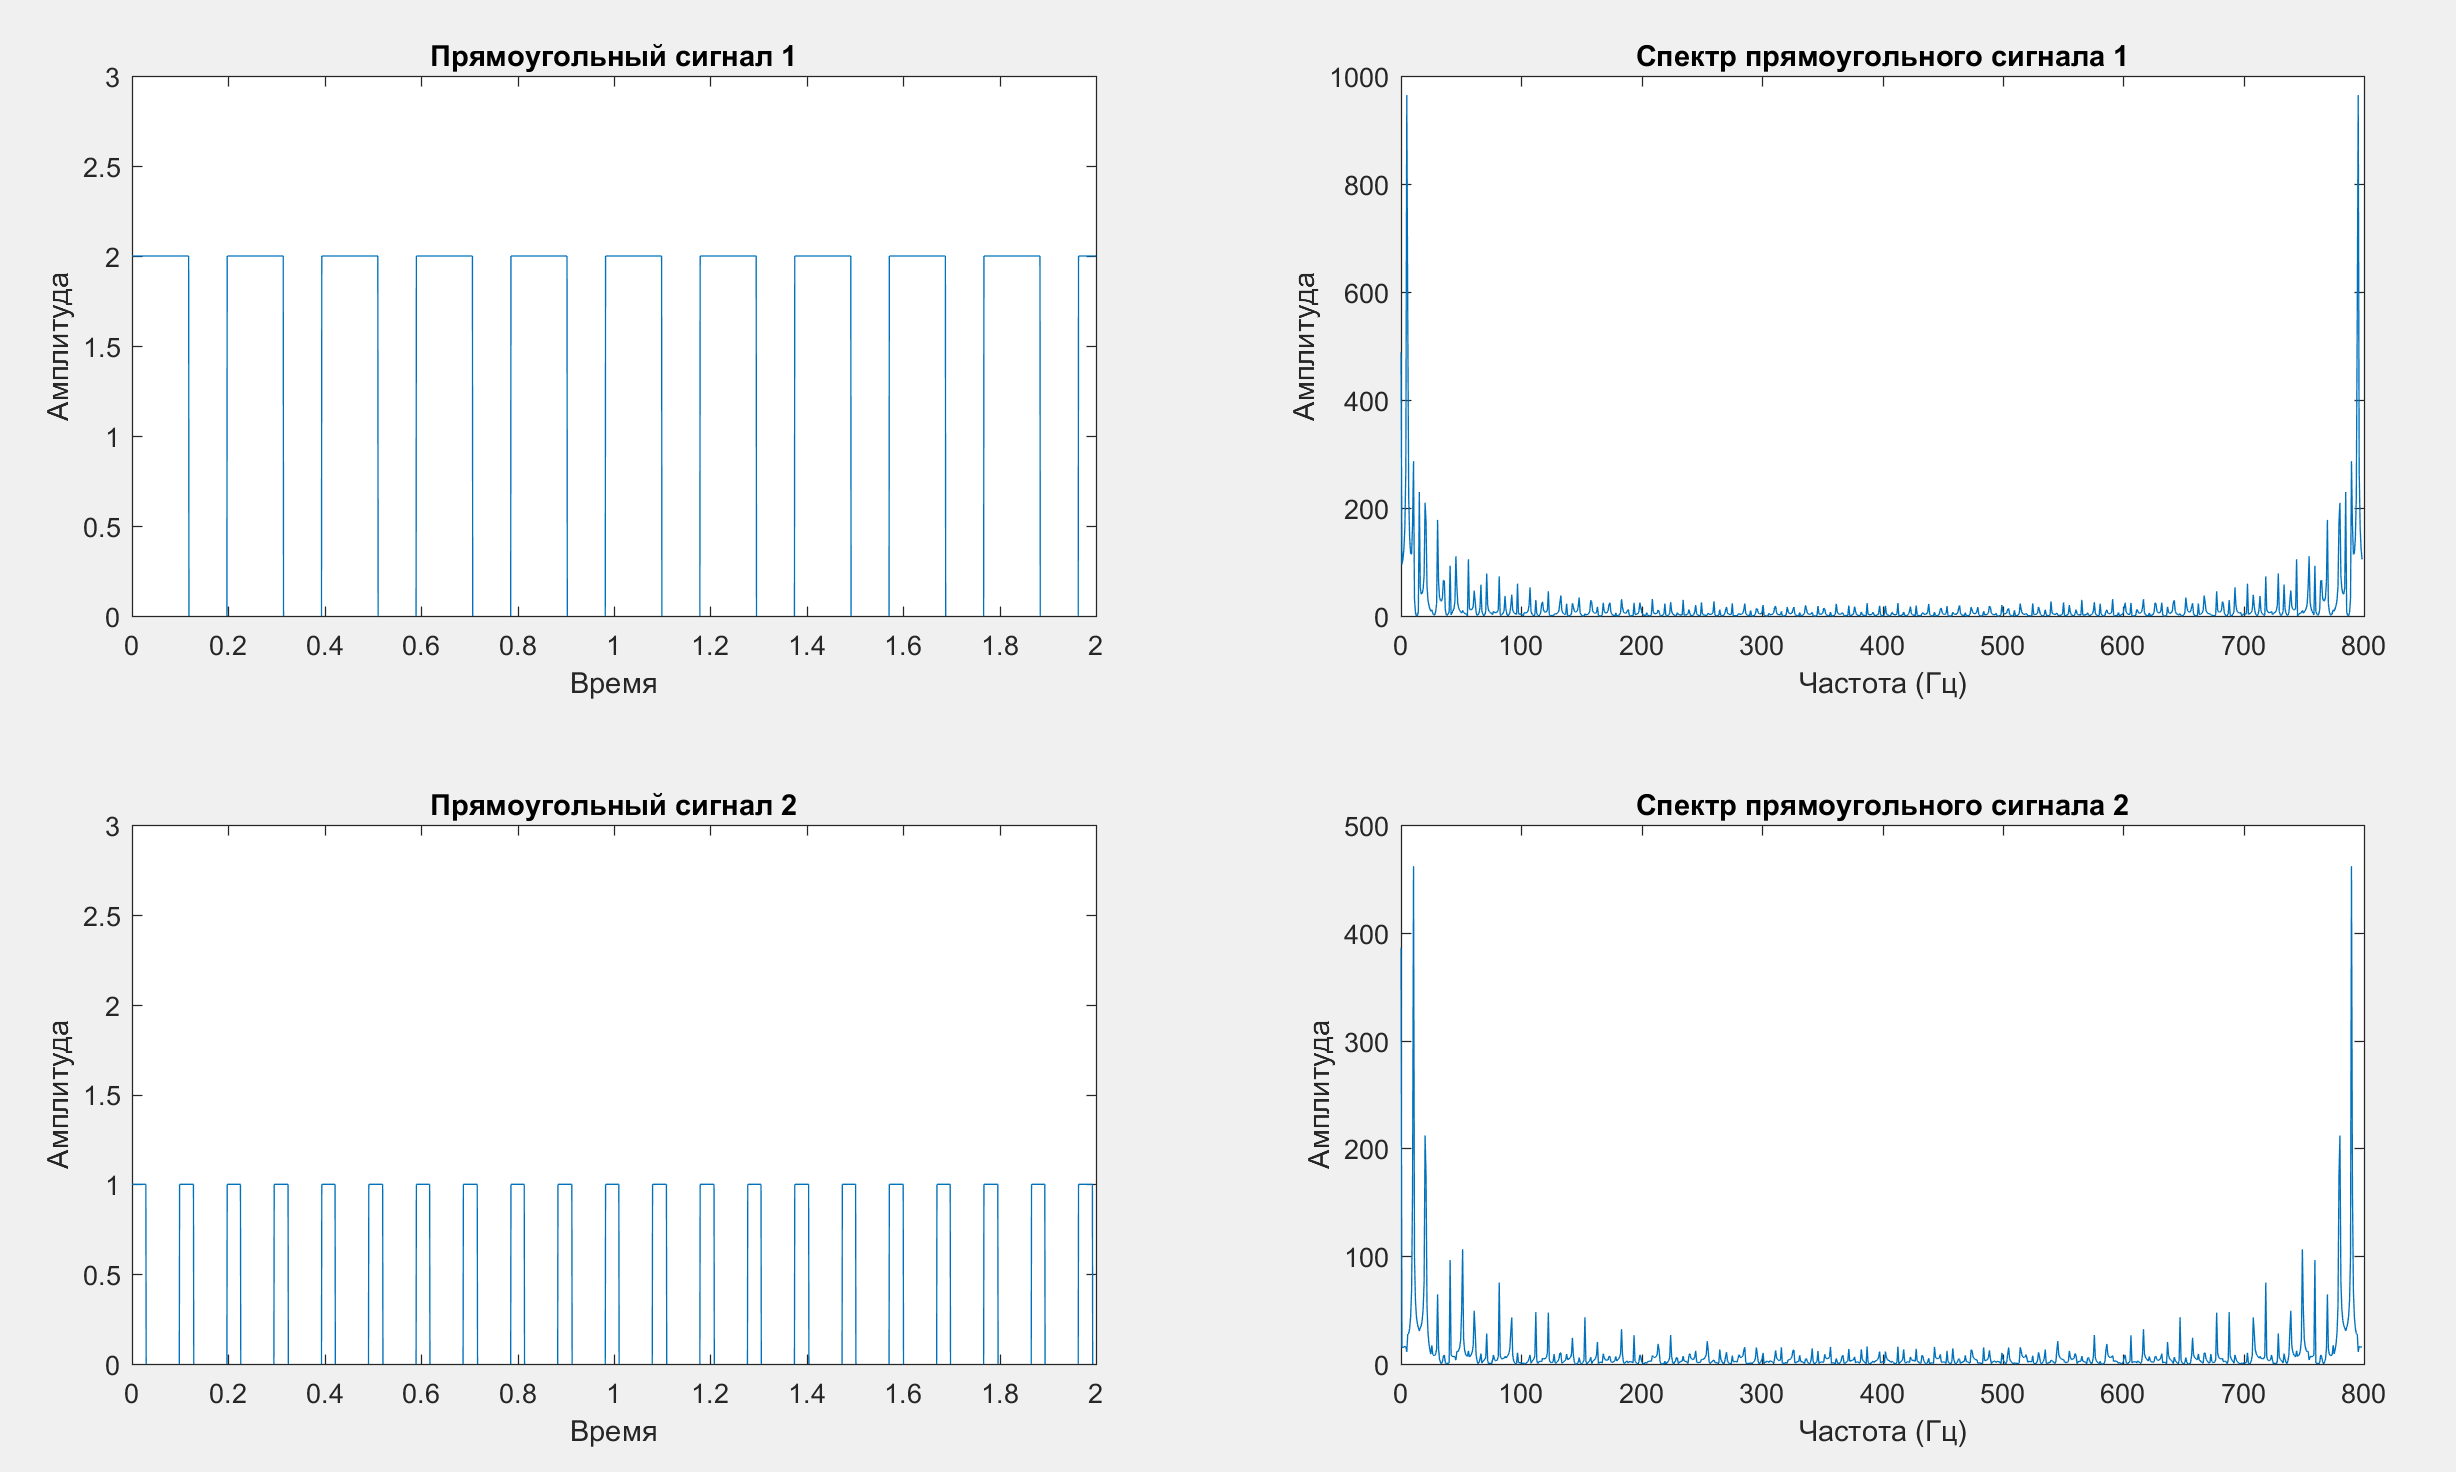
\includegraphics[width=0.9\linewidth]{square_out}}
\caption{Вывод прямоугольных импульсов и их спектров}
\end{figure}

\newpage
\subsection{Работаем в Simulink (синусоида)}
\label{sec:workSim1}

%Рисунок 9
\begin{figure}[h!]
\center{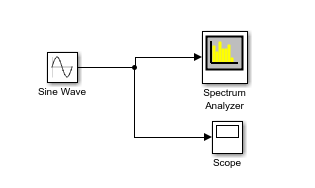
\includegraphics[width=0.9\linewidth]{simulink_sin}}
\caption{Cхема для синусоиды.}
\end{figure}

%Рисунок 10
\begin{figure}[h!]
\center{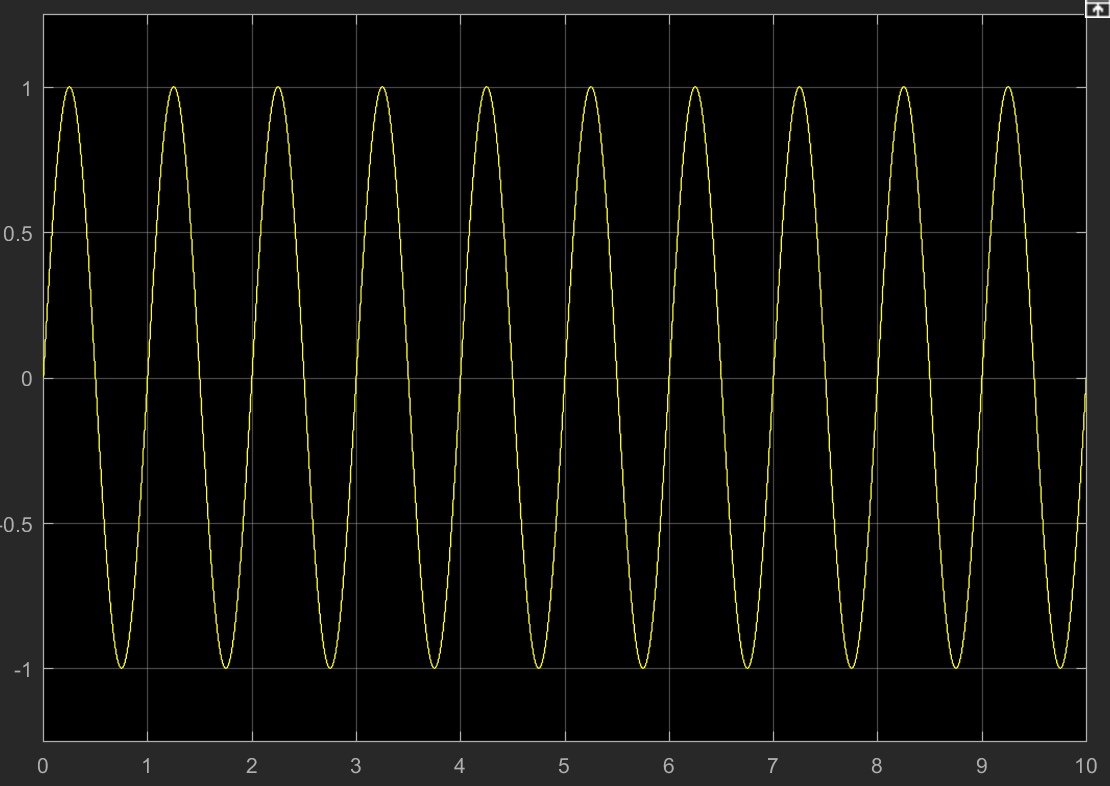
\includegraphics[width=0.9\linewidth]{sin_sim}}
\caption{Сигнал в Simulink.}
\end{figure}

%Рисунок 11
\begin{figure}[h!]
\center{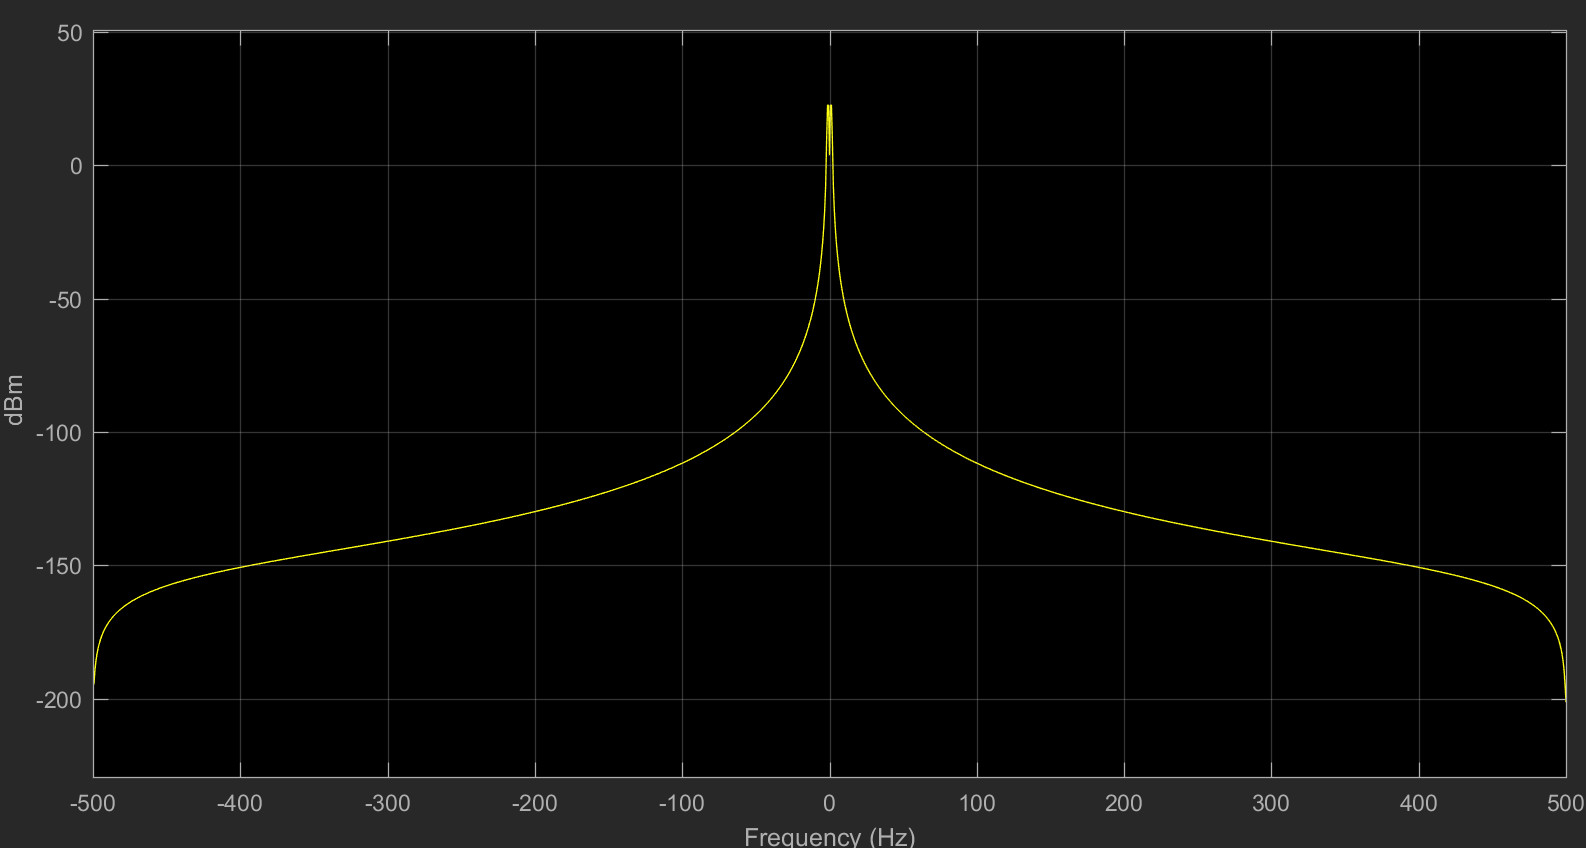
\includegraphics[width=0.9\linewidth]{sin_sp_sim}}
\caption{Спектр синусоиды в Simulink.}
\end{figure}

\clearpage
\newpage
\subsection{Работаем в Simulink (прямоугольный сигнал)}
\label{sec:workSim2}


%Рисунок 12
\begin{figure}[h!]
\center{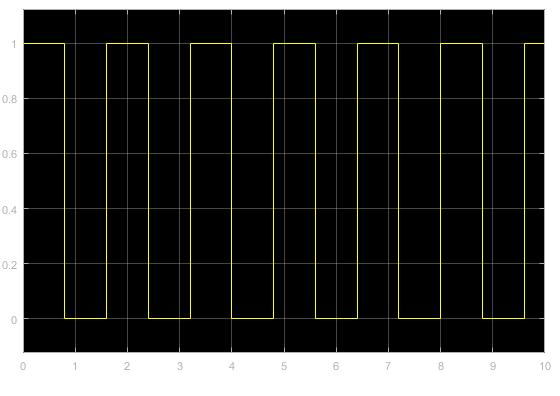
\includegraphics[width=0.9\linewidth]{square1-1600-800-0-00d1simulink}}
\caption{Прямоугольный сигнал в Simulink.}
\end{figure}

%Рисунок 13
\begin{figure}[h!]
\center{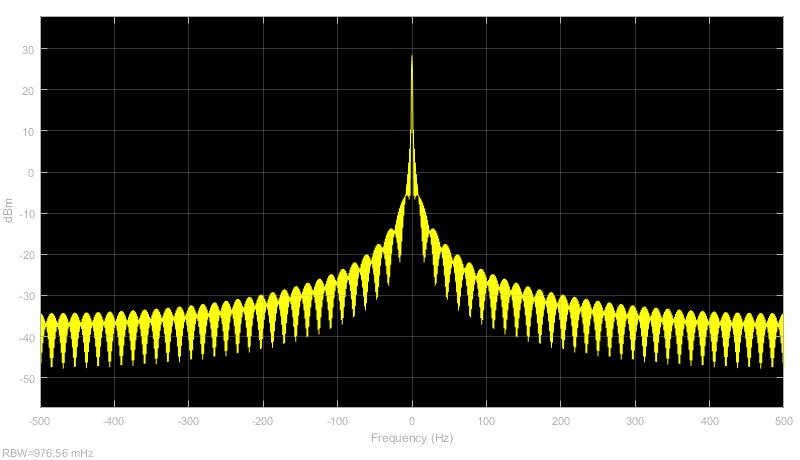
\includegraphics[width=0.9\linewidth]{square1-1600-800-0-00d1simulink_sp}}
\caption{Спектр прямоугольного сигнала в Simulink.}
\end{figure}

\clearpage
\newpage

\section{Вывод}
\label{sec:afterWork}
В ходе данной лабораторной работы мы познакомились со средствами генерации и визуализации простых сигналов. Были построены синусоида и прямоугольный импульсный сигнал в среде Matlab, а также в Simulink.

Классификация сигналов осуществляется на основании существенных признаков соответствующих математических моделей сигналов. Все сигналы разделяют на две крупных группы: детерминированные (значение сигнала можно определить в любой момент времени точно) и случайные. Детерминированные разделяются на периодические и непериодические(импульсые). К периодическим относят гармонические и полигармонические (сумма гармонических) сигналы. К непериодическим сигналам относят почти периодические и апериодические сигналы. Почти периодические сигналы близки по своей форме к полигармоническим. Они также представляют собой сумму двух и более гармонических сигналов (в пределе – до бесконечности), но не с кратными, а с произвольными частотами, отношения которых (хотя бы двух частот минимум) не относятся к рациональным числам. Апериодические сигналы составляют основную группу непериодических сигналов и задаются произвольными функциями времени.\\
\\

\end{document}